\documentclass[12pt,a4paper]{article}%
\usepackage[]{graphicx}\usepackage[]{color}
%% maxwidth is the original width if it is less than linewidth
%% otherwise use linewidth (to make sure the graphics do not exceed the margin)

%2multibyte Version: 5.50.0.2960 CodePage: 1252
\usepackage{amsfonts}
\usepackage{amssymb}
\usepackage[centertags]{amsmath}
\usepackage{graphicx}%
\usepackage{natbib}
\usepackage{color}
\usepackage[dvipsnames,svgnames*]{xcolor}
\usepackage{array}
\usepackage[hidelinks]{hyperref}
\usepackage[font=small,skip=5pt]{caption}
\usepackage[aboveskip=2pt]{subcaption}
\usepackage{amsmath}
\usepackage[]{algorithm2e}
\usepackage{amsthm}
\usepackage{url}
\usepackage{wasysym}
\usepackage{ulem}
\usepackage{afterpage}
\usepackage{bbm}
\setcounter{MaxMatrixCols}{30}
\providecommand{\U}[1]{\protect\rule{.1in}{.1in}}
\newtheorem{theorem}{Theorem}
\newtheorem{acknowledgement}[theorem]{Acknowledgement}
\newtheorem{axiom}[theorem]{Axiom}
\newtheorem{case}[theorem]{Case}
\newtheorem{claim}[theorem]{Claim}
\newtheorem{conclusion}[theorem]{Conclusion}
\newtheorem{condition}[theorem]{Condition}
\newtheorem{conjecture}[theorem]{Conjecture}
\newtheorem{corollary}[theorem]{Corollary}
\newtheorem{criterion}[theorem]{Criterion}
\newtheorem{definition}[theorem]{Definition}
\newtheorem{example}[theorem]{Example}
\newtheorem{exercise}[theorem]{Exercise}
\newtheorem{lemma}[theorem]{Lemma}
\newtheorem{notation}[theorem]{Notation}
\newtheorem{problem}[theorem]{Problem}
\newtheorem{proposition}[theorem]{Proposition}
\newtheorem{remark}[theorem]{Remark}
\newtheorem{solution}[theorem]{Solution}
\newtheorem{summary}[theorem]{Summary}
\setlength{\topmargin}{0in}
\setlength{\oddsidemargin}{0.1in}
\setlength{\evensidemargin}{0.1in}
\setlength{\textwidth}{6.5in}
\setlength{\textheight}{8.25in}
\numberwithin{equation}{section}
\title{Real Time Variational Density Forecasts}
\author{Nathaniel Tomasetti, Catherine Forbes and Anastasios Panagiotelis}
\begin{document}

\maketitle
\tableofcontents
\section{Introduction} \label{sec:Intro}
%label added to section for referencing later

Electricity prices have been subject to an extensive forecasting literature and is known to be extremely volatile. For the 2011-2015 period in Victoria the mean price per megawatt hour (mWh) was \$42.06, with 99\% of {\bf observations} less than \$100 {\bf per} % Try to minimize or not use shorthand mathematical notation in the introduction. 
mWh but on 39 {\bf occasions} the price spiked greater than \$1,000/mWh, reaching as high as \$9,974/mWh on November 29, 2012. 
% This is very precise information, but I think for an introduction it is better to try to keep it a bit more `big picture'. Perhaps even just writing in percentage terms will have more impact, rather than requiring the reader to work out if this difference is big or not. Then also you wouldn't need to units of measure in quite so many places. I'd even prefer not to have the abbreviation `mWh' here, but this is less critical. } 
For this reason market participants are increasingly interested in a predictive density forecast, as the probability that the price will rise above a particular threshold in the next time period is more important than the mean value. To calculate a suitably accurate predictive density the Bayesian methodology is to be adopted in this thesis, as it {\bf accounts for both } parameter and model uncertainty {\bf often} ignored {\bf by} frequentist methods. 
% I agree with Tas that it is better not to be so defensive at the outset. Better to justify that positives of Bayesian methods - in particular the use of prior information and the ability to handle complex, parameter-driven (state space) models. 
See \citet{Geweke2006} for a review on Bayesian forecasting and \citet{Gneiting2014} for density forecasting in general. 
% Sorry but I don't know why the references are not working for me!

% It might be useful to say something in the above about the connection between the predictive distribution, and the posterior distribution. Or just talk about distributions here, and then the connection to the forecast density can come in the next section.

Bayesian methods are computationally complex as they require integration over the set of {\bf unknowns, whether parameters or latent stochastic variables. This set is typically quite large for models used to model short term electricity load and price as there are} strong seasonal patterns {\bf in the data \citep{Taylor2003}.} {\bf While analytical integration is typically not feasible to obtain the predictive distribution for such models, however} there are a range of {\bf numerical and simulation-based} techniques available, {\bf for this purpose,} notably Markov Chain Monte Carlo (MCMC) methods. While {\bf it is often possible to demonstrate theoretical convergence of MCMC algorithms,} computation {\bf may be} slow for even moderately complex models. {\bf This} is problematic {\bf for when attempting to forecast} Electricity demand 
%demand? or price? or load? decide which you are going to talk about here, and only talk about that for now - check throughout.
in Victoria, {when realizations occur at} five minute {\bf intervals}. The predictive density for the next period's electricity load may not be available before it is observed.


Alternatives to MCMC include Variational Bayes (VB) {\bf methods, where the aim is} to replace the unknown true posterior distribution for a vector of {\bf unknowns}
% you can reduce to just $\theta$ below - but keep it general in the introduction
with a parametric approximation. {\bf The} Variational Bayes {\bf approach} will be explored {\bf in the thesis, to determine if it is a viable} alternative computation strategy to MCMC,
% comma added
in the context of {\bf modelling and short term forecasting of Victorian electricity load.}
% Unless you have something interesting to say about the time period - which could come later - there isn't any real need to mention the data period at this point. It could come in the last paragraph, however. 
{\bf In particular, we seek to understand the benefits gained in terms of the computational time required to obtain a VB approximate forecast distribution against the loss in statistical} 
% I think you need to use the spell checker!!
accuracy associated with the use of an {approximate posterior forecast distribution.} 
%

% You need a paragraph here detailing the outline of the rest of the paper, section by section.

\section{Bayesian Inference}

{\bf To facilitate the discussion, consideration is given to models where the unknowns may be summarized in a (finite) $k-$dimensional vector, denoted by $\theta.$ In this setting, given an observed time series, denoted by $y_{1:T}= \{y_{t}, t = 1, \dots T\}$, the Bayesian forecast distribution associated with time $t=T+1$ is characterized by the conditional density }
\begin{equation}
\label{predictive}
p(y_{T+1} | y_{1:T}) =\int p(y_{T+1}|y_{1:T},\theta) p(\theta|y_{1:T}) d\theta,
\end{equation}
{\bf where $p(\theta|y_{1:T})$ denotes the posterior density for $\theta$, given by}

\begin{equation}
\label{posterior}
 p(\theta | y_{1:T}) = \frac{p(y_{1:T}|\theta)p(\theta)}{\int_\theta p(y_{1:T}|\theta)p(\theta) d\theta}.
\end{equation}
% You can feel free to modify the above, but be sure to define all notation that you use.

% I think you need to expand this section a bit more - think about what you really need to say, and why.
Generally the {\bf analytical} solution to (\ref{posterior}), 
% comma added
{\bf and hence to (\ref{predictive}) will be unavailable.} 	% Can you say why? 
{\bf In this} section {\bf two alternative methods for computing the desired posterior distribution in (\ref{posterior}),  MCMC and VB, will be reviewed.}
% Since neither method is new, you are not `offering' them, just reviewing them.
% Can you extend this discussion to explain how to use MCMC and VB for (\ref{\predictive})?
{\bf In brief,} MCMC is used to create a sample from $p(\theta | y)$, {\bf with} any function {\bf of $\theta$ that is desired estimated from that sample. In contrast,} VB replaces $p(\theta | y)$ with an approximation,
%comma inserted
{\bf denoted by} $q(\theta | \lambda)$, where $\lambda$ is a vector of {\bf auxiliary} parameters associated with the approximation and not the model. 
% surely these $\lambda$ have something to do with the model??? Perhaps end the sentence with `approximation'. Also need to emphasize that $q(\theta|\lambda)$ is also a function of the data $y_{1:T}$.
For example, if $q(\theta | \lambda)$ is Gaussian,
%comma added
{\bf then} $\lambda$ would {\bf denote} the mean and variance {\bf parameters that characeterize this normal distribution for} $\theta$. Variational Bayes aims to choose the distribution $q(\theta | \lambda)$ such that the Kullback-Leibler divergence from $q(\theta | \lambda)$ to $p(\theta | y)$ is minimised.
% I have used `z' (as in `minimized') in my edits, not `s' (as in `minimised'), but you decide which you prefer and be consistent.
%So obviously now the values of the mean and variance will in fact depend on the data, and the Gaussian model will be selected due following consideration of at least a portion of the original, more complex model (via this minimization). So yes, the approximation and its parameters will, in some sense at least, depend on the model!

\subsection{Markov Chain Monte Carlo}

There are many types of MCMC {\bf algorithms, with arguably the simplest and most commonly used one being the} Gibbs sampler. {The Gibbs sampler algorithm} iteratively samples {\bf the components of the} $k$ dimensional parameter vector $\theta$ via {\bf each of} the {\bf so-called full} conditional distributions {\bf as follows,}
% I'm not sure you need the extra space above each equation - have not changed elsewhere but please consider
\begin{align}
&p(\theta_1 | \theta_2, \dots, \theta_k, y_{1:T}) \nonumber \\
&p(\theta_2 | \theta_1, \theta_3, \dots, \theta_k, y_{1:T}) \nonumber \\
&\vdots \nonumber \\
&p(\theta_k | \theta_1, \dots, \theta_{k-1}, y_{1:T}). \nonumber
\end{align}
% when you put a space after the equation, LaTeX thinks you are starting a new paragraph. Depending on the style you are using, this may generate a tab at the start of the next line, which you may not want - please be mindful of this, I have not corrected throughout.
{\bf Under mild regularity conditions (see, e.g., Tierney, 1994, Annals of Statistics) and with} enough iterations {\bf of the Markov chain that results from the Gibbs sampler,} these samples converge in distribution to $p(\theta | y)$ and can be used for inference. 
% The phrase `and can be used for inference' is a bit vague...
The computation time {\bf for each} iteration and {\bf the overall} number of iterations required for {\bf to accruately summarize the posterior distribution} is problem specific but typically increases with model complexity. 
% what do we know about model complexity? Can we just say it is $k$? Or do you want to highlight something more?


\subsection{Variational Bayes}

{\bf As discussed in Section \ref{sec:Intro}, a faster (albeit approximate)} alternative to MCMC is {\bf VB. This approach} introduces an approximating distribution {\bf $q(\theta | \lambda),$ with the choice of the functional form $q$ and subsequent auxiliary parameter $\lambda$ determined so that} the Kullback-Leibler (KL) divergence \citep{Kullback1951} from $q(\theta | \lambda)$ the true posterior $p(\theta | y)$ {\bf is minimised.} The KL divergence is defined by

\begin{equation}
\label{KL-def}
KL[q(\theta | \lambda) \hspace{.1cm}||\hspace{.1cm}p(\theta | y)] = \int q(\theta | \lambda) \ln \left( \frac{q(\theta | \lambda)}{p(\theta | y)}\right) d\theta.
\end{equation}
% no new para. Note it might be useful to add some space before and after the double vertical lines - to make the equation above easier to read. I have done but see what you think...I haven't changed elsewhere.
The KL divergence is a non-negative, asymetric %spelling
 measure of the discrepancy between $p(\theta | y)$ and $q(\theta | \lambda)$ that will {\bf be equal to} zero if and only if $p(\theta | y) = q(\theta | \lambda)$ almost everywhere \citep{Bishop2006}. Note that $KL[q(\theta | \lambda)||p(\theta | y)]$ can be expressed as

\begin{equation}
\label{KL-ELBO}
KL[q(\theta | \lambda)||p(\theta | y)] = \ln(p(y)) - \mathcal{L}(q, y)
\end{equation}

where $\mathcal{L}(q, y)$ is {\bf referred to} as the Evidence Lower Bound (ELBO), {\bf and is} defined by
% Can you give some intuition for why this is called the ELBO?
\begin{equation}
\label{ELBO}
\mathcal{L}(q, y) = \int_{\theta} q(\theta|\lambda) \ln (p(y, \theta|\lambda)) d\theta -  \int_{\theta} q(\theta|\lambda) \ln (q(\theta|\lambda)) d\theta.
\end{equation}

Since $\ln(p(y))$ is constant given $y$, maximising (\ref{KL-ELBO}) with respect to $q$ is equivalent to minimising (\ref{KL-def}). Maximising the ELBO is much more convenient than minimising the KL Divergence, {\bf as will} be shown in the following sections {\bf in the context of the} two major implementations of Varitaional %spelling
{\bf Bayes, namely} Mean Field Variational Bayes and Stochastic Variational Bayes. Each of these {\bf implementations} take advantage of the functional form of the ELBO, %comma inserted
and offer computationally efficient algorithms to find a $q(\theta | \lambda)$ that is optimal within a particular clas %spelling
of distributions. 

\subsubsection{Mean Field Variational Bayes} 

Mean Field Variational Bayes (MFVB) has origins in the physics literature \citep{Chandler1987} and restricts the class of distributions {\bf from which to select $q(\theta|\lambda)$} to the set of factorisable distributions,

\begin{equation}
\label{mf1}
q(\theta|\lambda) = \prod_i^k q_i(\theta_i | \lambda_i).
\end{equation}
% Again, Tas's comment here about not re-using $k$ for this
Each of the $k$ components $\theta_i$ may be a vector, but in most implementations are scalars. Each $\theta_i$ has an associated vector $\lambda_i$ which may be of a higher dimension than $\theta_i$. $\lambda_i$ is an auxillary parameter vector for the relevant factor $q_i$, which will be used in this section as shorthand notation for the distribution $q_i(\theta_i |\lambda_i)$. 

MFVB is widely used as it greatly simplifies maximisation of the ELBO (\citealp{Jordan1999}; \citealp{Bishop2006}), particularly in exponential family models \citep{Wainwright2008}.  Maximising the ELBO with respect to $q_i$ is as analytically involved as deriving the conditional distributions used in Gibbs based MCMC schemes, but the computation is simple. 
%It is not clear at this point what you mean by 'the computation'. Is it that the identification process is the same, but rather than sampling from the identified distribution, as in Gibbs sampling, here you will find the value of the parameter $\lambda_i$ to maximise the identified distribution (for fixed $y_{1:T}$ and fixed other parameters in $\theta$ other than $\theta_i$).
MFVB expresses (\ref{ELBO}) as a function of one $q_i$ only 
% This doesn't quite make sense to me. It must be that MFVB assumes that (\ref{ELBO}) can first be represented as some kind of product of similar expressions, one for each $i$, and then that the maximisation of (\ref{ELBO}) can be determined by maximising each of these expressions. We talked about this a bit last week - perhaps you can tease this out a bit more. Somehow the iteration comes in so as to achieve this maximum.
The final algorithm requires this {\bf process} to be repeated for each $i$ in $1, \dots, k$, {\bf until ...}.
%Some kind of convergence criterion is needed.
Using the notation $q_{\setminus i} = \prod_{j\neq i}q_j$, \citet{Attias1999} shows that 

\begin{equation}
\label{mf2}
q(\theta_i | \lambda_i) \propto\exp( \mathbb{E}_{q_{\setminus i}} [\ln(p(y,\theta))])
\end{equation}
% The sentence is missing a full stop, and also I'm not sure how it connects to everything else?
{\bf To illustrate the MFVB approach,} consider data $y_i$ for $i = 1, \dots, n$ generated {\bf independently} from a $\mathcal{N}(\mu, \sigma^2)$ distribution with {\bf independent marginal prior distributions given by} %It is $\mu$ that has a distribution, not $p(\mu)$ - changed here
$\mu \sim \mathcal{N}(\gamma, \lambda)$ and $\sigma^2 \sim Inv.Gamma(\alpha, \beta)$. It can be shown that
% I think you need some $\lambdas$ below? Also would be worthwhile to  explain or show why these are the correct MFVB distributions...or at least be able to say something about it during your presentation.

\begin{equation}
\label{mf3}
q(\mu) \propto \exp \left\{ \frac{-(n\lambda + \mathbb{E}(\sigma^{-2}))}{2\lambda\mathbb{E}(\sigma^{-2})} \left( \mu - \frac{\mathbb{E}(\sigma^{-2})\gamma + \lambda \sum_{i=1}^{n} y_i}{n \lambda + \mathbb{E}(\sigma^{-2})} \right)^2 \right\}
\end{equation}

and

\begin{equation}
\label{mf4}
q(\sigma^2) \propto \sigma^{-2(n/2 + \alpha + 1)} \exp \left\{ \frac{ -1/2(\sum_{i=1}^{n}y_i^2 + n\mathbb{E}(\mu^2) - 2\sum_{i=1}^{n} y_i \mathbb{E}(\mu)) - \beta}{\sigma^2} \right\}.
\end{equation}

It is evident that $q(\mu | \lambda) \sim \mathcal{N}(\tilde{\gamma}, \tilde{\lambda})$ and $q(\sigma^2 | \lambda) \sim Inv.Gamma(\tilde{\alpha}, \tilde{\beta})$. The parameters $\lambda = (\tilde{\gamma}, \tilde{\lambda}, \tilde{\alpha}, \tilde{\beta})'$ can be found 
% how? I think you are just looking at the equations and `identifying' these guys, but it would be usefult to explain this. At least you have to mention something about how to evaluation, e.g. $E(\sigma^{-2})$ in $q(\mu | \lambda) \sim \mathcal{N}(\tilde{\gamma}, \tilde{\lambda})$ to get that $\tilde{\gamma} = \frac{\alpha / \beta \gamma + \lambda \sum_{i=1}^{n} y_i} {n \lambda + \alpha / \beta}$. Same for the other parameters too..
by the set of mean field equations:

\begin{align}
\tilde{\gamma} &= \frac{\alpha / \beta \gamma + \lambda \sum_{i=1}^{n} y_i} {n \lambda + \alpha / \beta} \label{mf5} \\ 
\tilde{\lambda} &= \frac{n \alpha / \beta}{n \lambda + \alpha / \beta} \\
\tilde{\alpha} &= \frac{n}{2} + \alpha \\
\tilde{\beta} &= \frac{1}{2} \left(\sum_{i=1}^{n} y_i^2 + n(\tilde{\gamma}^2 + \tilde{\lambda}) - 2 \sum_{i=1}^{n} y_i \tilde{\gamma} \right) + \beta. \label{mf6}
\end{align}.

As there is a circular dependence in these equations an algorithm that cycles through each auxillary %spelling
parameter until convergence to some pre-specified threshold %need to give some definition of this
is required.

%Paragraph moved below

Matching distributions in this way is a very similar method to finding the posterior conditional distribution, $p(\theta_i | y, \theta_{\setminus i}),$ %parenthesis and comma added, but I think this is different notation to what you used before - needs to be the same!
{\bf for example} in a Gibbs {\bf sampling} MCMC scheme, with dependence on other parameters replaced by their expectations. The optimal approximating family for $\theta_i$, $q(\theta_i | \lambda_i)$, will come from the same distributional family as the conditional distribution $p(\theta_i | \theta_{j \neq i}, y)$. % full stop added. Isn't this true, regardless of whether we can recognize the form or not? 
if it exists in a recognisable form such as the exponential family. % have left this for you to resolve...

% moved paragraph to here
In the event that {\bf the form of the distribution in} (\ref{mf2}) is {\bf unrecognisable,} a further approximation {\bf may} be used {\bf by} substituting in another distribution {\bf to replace} the problematic $\tilde{q_i(\theta_i|\lambda_i)}.$ One {\bf approach, given by \citet{Friston2006},} uses a Laplace {\bf approximation, substituting} a Gaussian distribution for {\bf the} unrecognizable $q_i(\theta_i | \lambda_i)$. {\bf The} only requirement {\bf for this approach} is that the substitute {\bf have} an expectation 
% expectations? don't we need both of the first two moments? 
that is a tractable function 
% that are tractable functions? 
of {\bf the} parameters to be used for other parameters in (\ref{mf2}). 
{\bf This} secondary level of {\bf approximation} is analogous to the requirement of a Metropolis-Hastings-within-Gibbs step in MCMC to handle unrecognisable distributions. % I really like this analogy, and it will help your audience understand what is going on. But to make it work, you should have explained MHwithinGibbs earlier.



% Moved revised sentence down to here. But now you'll need to work this in with the following paragraph!
In the event that {\bf the form of the distribution in} (\ref{mf2}) is {\bf unrecognisable,} a further approximation {\bf may} be used {\bf by} substituting in another distribution {\bf to replace} the problematic $\tilde{q_i(\theta_i|\lambda_i)}.$ One {\bf approach, given by \citet{Friston2006},} uses a Laplace {\bf approximation, substituting} a Gaussian distribution for {\bf the} unrecognizable $q_i(\theta_i | \lambda_i)$. {\bf The} only requirement {\bf for this approach} is that the substitute {\bf have} an expectation 
% expectations? don't we need both of the first two moments? 
that is a tractable function 
% that are tractable functions? 
of {\bf the} parameters to be used for other parameters in (\ref{mf2}). 


\vspace{5mm}

% You have not really fully explained how this algorithm below fits with what is above?? A single sentence might be sufficient.
{\bf Once the approximation has been identified, the algorithm required to find the ELBO is} known as a coordinate ascent algorithm. %full stop
{\bf This algorithm} is described below {\bf in the case} where $\lambda$ is a $p$ dimensional vector. %why change from $k$ to $p$? need to keep consistent notation throughout. 
%We have discussed these algorithms already, and I have nothing more to add now

\vspace{2mm}

\begin{algorithm}[H]
 \SetKwInOut{Input}{Input}
 \Input{Log Joint Density}
 \KwResult{Mean Field Approximation}
 Use (\ref{mf3}) to match each $q(\theta_i|\lambda_i)$ to a tractable distribution or substitute a further approximation if neccesary.\;
 Derive the set of mean field equations, such as (\ref{mf5}) - (\ref{mf6}).\;
 Initialise $\lambda$ randomly. \;
 \While{Not converged}{
  \For{$i =  1$ \KwTo $k$}{
      Hold $\lambda_{j \neq i}$ fixed\;
      Update $\lambda_i$ using the relevant mean field equation.
     }
 }
 \caption{Coordinate Ascent for MFVB}
  \label{alg:algorithm1}
\end{algorithm}

\subsubsection{Stochastic Variational Bayes}



Restricting the approximating distribution to a factorisable family may be unsatisfactory in many applications where the dependence between parameters is important, as in the AR(2) model where Figure \ref{MCMCplot} shows strong dependence between $\phi_1$ and $\phi_2$. Without factorisation the simple method to maximise the ELBO as in MFVB is unavailable. \citet{Paisley2012} and \citet{Ranganath2014} have adapted a gradient ascent algorithm for use in Variational Bayes, resulting in what is known as Stochastic Variational Bayes (SVB).

The algorithm for SVB iteratively takes the  derivative of $\mathcal{L}(q(\theta | \lambda), y)$ in (\ref{ELBO}) with respect to $\lambda$ and the following updating step is applied until the ELBO converges to a maximum.

\begin{equation}
\label{SGA1}
\lambda^{(m+1)} = \lambda^{(m)} + \rho^{(m)} \nabla_{\lambda} \mathcal{L}(q(\theta | \lambda^{(m)}), y),
\end{equation}

where $\nabla_{\lambda}\mathcal{L}(q(\theta | \lambda^{(m)}), y)$ is the vector of partial derivatives of $\mathcal{L}(q(\theta | \lambda^{(m)}), y)$ with respect to each element of $\lambda$. This update requires some initial values $\lambda^{(0)}$ and a sequence $\rho^{(m)}, m = 1, 2, \dots$ known as the learning rate. If $\rho^{(m)}$ is chosen to satisfy the following conditions the algorithm is guaranteed to converge to a local maximum \citep{Robbins1951}.

\begin{align}
\sum_{m=1}^{\infty} \rho^{(m)} &=  \infty \\
\sum_{m=1}^{\infty} (\rho^{(m)})^2 &<  \infty.
\end{align}

Whilst a global maximum is desired, the ELBO is a high dimensional problem specific function that makes finding the global maximum extremely difficult and often only a local maximum can be found. One option to alleiviate this problem is to start the algorithm at a range of initial values choose the converged value with the highest maximised ELBO and hence lowest KL divergence to the true posterior 

SVB can find only the optimal values for $\lambda$ that are optimal for a distributional family $q$ that is specified by the user. To run SVB many choices of $q$ may be used and one selected on the basis of the highest ELBO. $q(\theta | \lambda)$ is restricted to the family of distributions that satisfy the condition that the order of differentation of the ELBO with respect to $\lambda$ and integration with respect to $\theta$ are interchangable, and SVB can only be applied to models where the log likelihood for $y$ is able to be evaluated. Given these conditions \citet{Ranganath2014} showed that a Monte Carlo estimate of the derivative of the ELBO can be taken by

\begin{equation}
\label{SGA2}
\nabla_{\lambda}\mathcal{L}(q(\theta | \lambda^{(m)}) \approx \frac{1}{S}\sum_{s=1}^{S} \nabla_{\lambda} [\ln(q(\theta_s | \lambda^{(m)}))] (\ln (p(y, \theta_s)) - \ln(q(\theta_s | \lambda^{(m)})))
\end{equation}

where $s = 1, \dots, S$ indicates simulations from $q(\theta | \lambda^{(m)})$.

\citet{Duchi2011} introduced the AdaGrad algorithm which can be implemented within SVB to control $\rho^{(m)}$. AdaGrad allows each $\lambda_i$ to have an independent $\rho^{(m)}_i$ that is inversely proportional to the gradient, so $\lambda$ takes bigger steps in flat regions and smaller steps in steep regions. 

Let 

\begin{equation}
\label{SGA3}
G_i^{(m)} = \sum_{j = 1}^{m} \left(\nabla_{\lambda_i}\mathcal{L}(q(\theta | \lambda^{(m)})\right)^2,
\end{equation}

then each component's learning rate is defined as

\begin{equation}
\label{SGA4}
\rho^{(m)}_i = \eta \left(G_i^{(m)}\right)^{-1/2}
\end{equation}

for some tuning parameter $\eta$.

The resulting Stochastic Gradient Ascent algorithm proceeds below with a $p$ dimensional $\lambda$ vector.

\begin{algorithm}[H]
 \SetKwInOut{Input}{Input}
 \Input{Log Joint Density, Approximation family q}
 \KwResult{Variational Approximation}
 Initialise $\lambda$\;
 \While{Not converged}{
  Simulate $\theta^s$ for $s = 1, \dots S$ from $q(\theta|\lambda^{(m)})$\;
  \For{$i =  1$ \KwTo $p$}{
      Calculate $\nabla_{\lambda_i}$ from (\ref{SGA2})\;
      Update $G_i^{(m)}$ and $\rho^{(m)}_i$ from (\ref{SGA3}) and (\ref{SGA4})\;
      }
  Update $\lambda^{(m+1)}$ from (\ref{SGA1})\;
  Set $m = m + 1$\;
 }
 \caption{Stochastic Gradient Ascent for SVB}
  \label{alg:algorithm2}
\end{algorithm}


\subsection{Vine Copulas}
% I won't add too many more to Tas's comments, except to remind you to take the sorts of critiques I have made above and try to apply them here - be clear about what you are saying, don't leave out so many words and use that spell checker :-)

Armed with an algorithm to find the Variational Bayes optimal paramerters $\lambda$ for a distribution $q$, there is a requirement to have a distribution $q$ that is itself optimal. Copulas are a flexible tool for constructing these distributions, as they allow the dependence structure between parameters to be fit independently from the marginal distributions. \citet{Sklar1959} proves that any joint probability distribution can be written as the product of the marginals and a copula function,

\begin{equation}
\label{vc1}
p(\theta_1, \dots, \theta_k) = p(\theta_1) \dots p(\theta_k) c(P(\theta_1), \dots, P(\theta_k))
\end{equation}

where $p(\theta)$ is a pdf, $P(\theta)$ is a cdf, and $c(\cdot)$ is a copula. 

\citet{Joe1994} introduces the vine copula, a technique to factorise a high-dimensional copula into a set of bivariate copulas in a similar way to the factorisation of a joint distribution into a marginal and conditional distribution, for example

\begin{equation}
\label{vc2}
c(P(\theta_1), P(\theta_2), P(\theta_3)) = c(P(\theta_1), P(\theta_2)) \cdot c(P(\theta_1), P(\theta_3)) \cdot c(P(\theta_2), P(\theta_3) | P(\theta_1)).
\end{equation}

A copula for a $k$ dimensional $\theta$ can be replaced with $k(k-1)/2$ bivariate copulas arranged in a vine copula, greatly increasing the amount of flexibility available to fit a distribution. However there are $O(k!)$ ways to factorise the full copula and choose a family for each bivariate copula, so without detailed problem specific information the application of a vine copula to Stochastic Variational Bayes is difficult. \citet{Tran2015} implements Variational Bayes with a vine copula in what they call Copula Variational Bayes, but the dimension of $\theta$ was small in that case allowing an exhaustive search for the vine copula that maximised the ELBO. 

Given a sample of $\theta$, \citet{Diimann2013} provide an algorithm to select the best vine factorisation by maximising Kendell's Tau, and the best family for each bivariate copula by maximising an information criterion such as AIC. In the real-time forecasting models used for electricity load demand, MCMC samples of the posterior distribution are available, though often immediately out of date. The approach used in this thesis is to run an MCMC algorithm, thin the resulting draws until they are effectively independent, choose an optimal family for each marginal distribution by AIC, then run (Vine copula algorithm here) to infer an optimal vine copula. This results in an approximating distribution $q(\theta | \lambda)$ that can then be used in an SVB algorithm to update $q(\theta | \lambda)$ as more observations become available. MCMC can be ran simultaenously and the resulting sample can be used to check if the distribution $q$ should be changed. 

\subsection{Applying Stochastic Variational Bayes}

Using the approach described in {\bf Section} 2.3,
% When referring to a specific section, use a capital letter. When referring generally to `this section' or `later sections', etc, use lower case.
an application of VC algorirhtm to the MCMC draws obtained in {\bf Section} 2.1 % You can check the rest
found the following distribution to be optimal, {\bf according to the standard Akaike Information Criterion (AIC)}.

\begin{itemize}
\item $q(\phi_1)$ - Gaussian marginal
\item $q(\phi_2)$ - Gaussian marginal
\item $q(\sigma^2)$ - Inverse Gamma marginal
\item $c(Q(\phi_1), Q(\phi_2))$ - Gaussian copula
\item $c(Q(\phi_1), Q(\sigma^2))$ - Independent
\item $c(Q(\phi_2), Q(\sigma^2) | Q(\phi_1))$ - Independent
\end{itemize}

Figure \ref{VBfit} shows that Stochastic Variational Bayes (blue) fit the MCMC (red) sample very closely.

\begin{figure}[h]
\centering
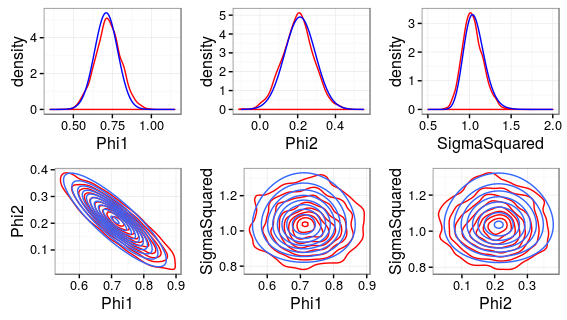
\includegraphics[scale = 0.5]{VBfit.png}
\caption{The fit of an SVB algorithm (red) compared to MCMC (red) for the AR(2) model described in section 2.1. SVB resulted in an almost identical posterior to MCMC, requiring around one hundredth of the runtime for MCMC.}
\label{VBfit}
\end{figure}

\section{Electricity Load Forecasts}
\subsection{Motivation}

The literature for electricity forecasting is wide, and contains models based on many different fields, such as game theory, time-series modelling and neural networks, see \citet{Weron2014} for a recent review. Density forecasting for short term electricity load has had less attention, with \citet{Fan2012} and \citet{He2016} 
% one of the disadvantages of the automatic citations is that the formatting isn't quite as I would expect. Perhaps a different bibliographical style would be better. In Econometrics, we typically list the full set of authors names the first time a paper having 3 (sometimes 4) or more authors, and then if cited again use the `et al.' convention. Also, the `et al.' should be in italics. But this is minor for now...
being notable examples, which used boot strapping and quantile regression respectively to generate forecast densities. Both of these approaches create forecast densities that are conditioned on the model and estimated parameters being correct, while the Bayesian approach used in this thesis can average over parameter and model uncertainty leading to a more accurate forecast density. This thesis also aims to re-estimate the model after each data point is observed to fully take advantage of any extra information on changes in parameters and thus further increase the accuracy of the forecast density. 

Half hourly electricity load data for Victoria, Australia has been collected % You need to report where you got the data from. You didn't collect it yourself, which is how it reads!
 for the 2011-2015 period, and is plotted in Figure \ref{loadplot}. The time series displays strong seasonal characteristics, with a yearly, day of week, and time of day pattern. Electricity load is strongly dependent on temperature, with high load experienced on both very cold and very hot days. In summer periods, load is often low but shows extreme volatility, while load slowly rises then falls in winter and displays significantly less volatility. 

The electricity market in Victoria operates by market participants sending electricity bid and offers for each five minute period to  AEMO, a centralised market operator. AEMO then determines the dispatch price and load for that five minute period, and determines the final spot price participants pay for each half-hour period by averaging the six five minute dispath% spelling
 prices in that half-hour. Market participants are allowed to revise bids and offers at any point before dispatch. The electricity supply curve is strongly J shaped, as coal generators are able to provide a large load cheaply but if demand exceeds this level the price spikes as other generators must be brought online expensively. These characteristics of the electricity market leads to a large amount of volatility in prices demonstrated by Figure \ref{rrpplot}. The seasonal effects of the load data are also present in prices, but these effects are dominated by irregular spikes as high as \$9,974/mWh, compared to a four year mean of \$42/mWh.

\begin{figure}[h]
\centering
\includegraphics[scale = 0.5]{load_timeseries.png}
\caption{Half hourly load data measured in megawatt hours for Victoria from January 1 2011 to December 31 2015. The yearly pattern is characterised by a low median load with regular spikes in summer and a more consistent sine curve in winter. Note: Replace with daily average to make the pattern clearer?}
\label{loadplot}
\end{figure}.


\begin{figure}[h]
\centering
\includegraphics[scale = 0.5]{RRP_timeseries.png}
\caption{Half hourly price data for Victoria from January 1 2011 to December 31 2015. The price shows a strong time of week and time of day seasonal effect in the low price periods, and has irregular spikes.}
\label{rrpplot}
\end{figure}.

\subsection{Exponential Smoothing}

\citet{Taylor2003} explores the seasonal properties of minute-by-minute electricity demand in the United Kingdom and introduces a double seasonal Holt-Winters exponential smoothing model with daily and weekly effects described by (\ref{ds-hw1})-(\ref{ds-hw4}). Yearly effects are omitted as their inclusion requires a large number of latent states to be estimated. This model is later verified 
% Verified is a very strong word. I would say these authors have provided empirical support that the model is superior
in \citet{Taylor2008} as superior to other common time-series models for very short-term load forecasting.

\begin{align}
y_t &= l_{t-1} + d_{t-m_1} + w_{t-m_2} + e_t \label{ds-hw1} \\
l_t &= \alpha (y_t - d_{t-m_1} - w_{t-m_2}) + (1 - \alpha)l_{t-1} \label{ds-hw2}\\
d_t &= \delta (y_t - l_{t-1} - w_{t-m_2}) + (1 - \delta)d_{t-m_1} \label{ds-hw3} \\
w_t &= \omega (y_t - l_{t-1} - d_{t-m_1}) + (1 - \omega)w_{t-m_2} \label{ds-hw4}
\end{align}

where $m_1$ and $m_2$ are the lengths of the daily and weekly cycle, restricting the smoothing parameters $\alpha, \delta, \omega$ to lie in $(0, 1)$. This can be rewritten as a single source of error state-space model, {\bf as per \citep{Snyder1985},  as follows}

\begin{align}
y_t &= l_{t-1} + d_{t-m_1} + w_{t-m_2} + e_t \label{ds-hw-ssoe1} \\
l_t &= l_{t-1} + \alpha e_t \label{ds-hw-ssoe2} \\
d_t &= d_{t-m_1} + \delta e_t \label{ds-hw-ssoe3} \\
w_t &= w_{t-m_2} + \omega e_t \label{ds-hw-ssoe4}. 
\end{align}

% Now I think you should really explain what `single source of error' means, and why it is useful (it means you have the likelihood in closed form, except for the initializing state variables and parameters - which together would make up your $\theta$ vector).  Also you can identify what the `state' at time $t$ is
The unknown parameters are $\theta = (\alpha, \delta, \omega)', \sigma^2$ and $b_0 = (l_0, d_0, \dots, d_{-(m_1 - 1)}, w_0, \dots, w_{-(m_2 - 1)})'$ a $m_1 + m_2 + 1$ length vector of the initial states of the latent variables. 
\citet{Forbes2000} derives the marginal distribution $p(\theta | y)$ and notes that, conditioned on a draw of these parameters, the remaining unknown parameters can be sampled as a Bayesian linear regression problem. This method involves inverting a matrix that is singular using the parameterisation described by (\ref{ds-hw-ssoe1}) - (\ref{ds-hw-ssoe4}), but restricting the latent parameters via

\begin{align}
d_t &= - \sum_{i=1}^{m_1-1} d_{t-i} \\
w_t &= - \sum_{i=1}^{m_2-1} w_{t-i}
\end{align}

avoids this problem. The resulting model is described by

\begin{align}
y_t &= l_{t-1} - \sum_{i = 1}^{m_1 - 1}d_{t-i} - \sum_{i = 1}^{m_2 - 1}w_{t-i} + e_t \label{ds-hw-rp1} \\
l_t &= l_{t-1} + \alpha e_t \label{ds-hw-rp2} \\
d_t &= - \sum_{i = 1}^{m_1 - 1}d_{t-i} + \delta e_t \label{ds-hw-rp3} \\
w_t &= - \sum_{i = 1}^{m_2 - 1}w_{t-i} + \omega e_t \label{ds-hw-rp4}.
\end{align}

\citet{Forbes2000} recommends numerical integration of the marginal posterior density of $\theta$,

\begin{equation}
\label{exp-sm-marginal}
p(\theta | y_{1:T}) \propto \left| \widetilde{X}' \widetilde{X} \right|^{-1/2} \tilde{s}^{-(T-(m_1 + m_2 - 1))} p(\theta),
\end{equation}

where $\widetilde{X}$ and $\tilde{s}$ are functions of $\theta$ and $y$. The problems with using this method in our model are two-fold: repeating a three dimensional numerical integrion each time a new data point is observed within the five minute window is not feasible difficult, and the $T$ in the exponent makes most evalutions of $p(\theta | y_{1:T})$ computationally zero when $T$ is large. 

\begin{itemize}
\item Should try and get an exponential smoothing MCMC working using Metropolis-Hastings for $\theta$. Log densities help with the $T$ being too large problem but the grid is too large for numerical integration to be a good idea.
\end{itemize}

% You need a concluding paragraph, in addition to the timeline below.
\section{Timeline}
\begin{itemize}
\item Put something here eventually
\end{itemize}

\bibliographystyle{asa}
\bibliography{references}

\end{document}
\grid
